\newpage
\setcounter{figure}{0}

\section{Rezultati} % (fold)
\label{sec:Rezultati}

U ovom poglavlju prikazani su rezultati rada razvijenog programa za
prepoznavanje statičnog znaka iz snimke prometnice vozila u pokretu.  Za ispitivanje funkcionalnosti metode odabrana su tri scene vožnje
s tri različita znaka koje program treba pronaći. Znakovi su 
prikazani na
slici~\ref{fig:znak}, a scene vožnje su snimljene na osječkoj
obilaznici i prikazane na slikama~\ref{fig:scena.png} i \ref{fig:scena2}. Slika~\ref{fig:scena2} također prikazuje prozor
regije interesa odabrane za pronalazak znaka te sliku matrice
rezultata izračunatih nad trenutnoj regiji interesa i učitanim znakom. 


\begin{figure}[!htb]
\minipage{0.3\textwidth}
\endminipage\hfill
\minipage{0.12\textwidth}
    \includegraphics[width=\linewidth]{figures/znak2.jpg}
\endminipage\hfill
\minipage{0.12\textwidth}
    \includegraphics[width=\linewidth]{figures/znak3.jpg}
\endminipage\hfill
\minipage{0.12\textwidth}
    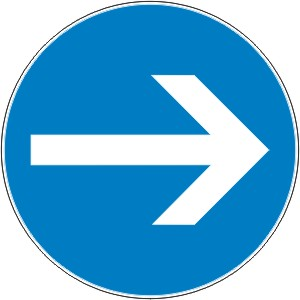
\includegraphics[width=\linewidth]{figures/znak.png}
\endminipage\hfill
\minipage{0.3\textwidth}
\endminipage\hfill
\caption{Prikaz korištenih znakova - obvezan smjer kretanja u desno (lijevi znak), 
obilaženje s obje strane (srednji znak), prvenstvo prolaza (desni znak)}
\label{fig:znak}
\end{figure}

\begin{figure}[!htb]
\minipage{0.475\textwidth}
    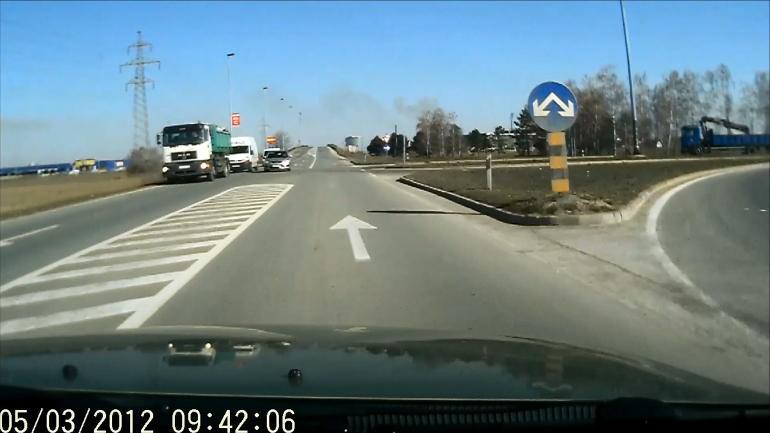
\includegraphics[width=\linewidth]{figures/scena1.png}
\endminipage\hfill
\minipage{0.05\textwidth}
\endminipage\hfill
\minipage{0.475\textwidth}
    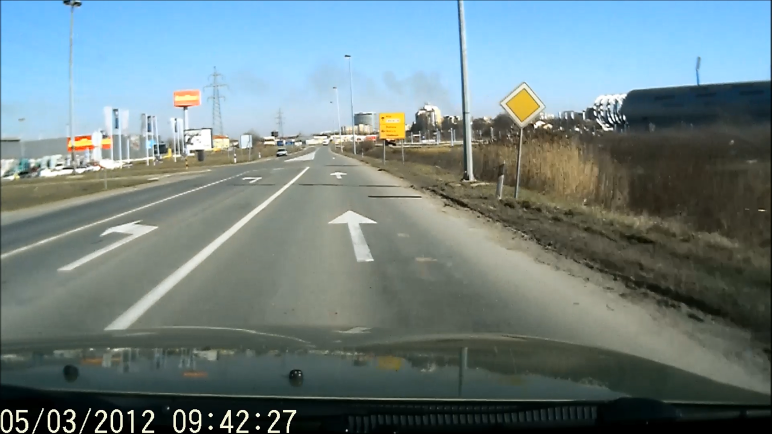
\includegraphics[width=\linewidth]{figures/scena3.png}
\endminipage\hfill
\caption{Prikaz testirane scene vožnje obilaženje s obje strane (lijevo) i
prvenstvo prolaza (desno)}
\label{fig:scena.png}
\end{figure}

\begin{figure}[h]
\centering
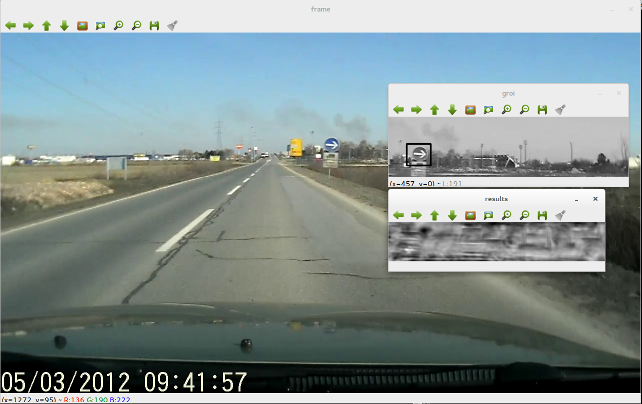
\includegraphics[scale=0.5]{figures/scena2.png}
\caption{Prikaz testirane scene vožnje obvezan smjer kretanja u desno}
\label{fig:scena2}
\end{figure}


\newpage
\subsection{Prikaz rezultata} % (fold)
\label{sub:Prikaz rezultata}

Rezultati su prikazani na slikama s dva prozora. U gornjem prozoru 
"groi" prikazana je regija interesa sa scene unutar koje algoritmom usporedbe
tražimo znak. Regija interesa je odabrana na temelju pretpostavke da će
pozicija znaka bit s desne strane učitane scene. Također regija interesa
se definira kako bih se smanjila količina podataka koju algoritam mora
obraditi. U donjem prozoru "results" prikazana je matrica rezultata koju metoda
koristi za pronalazak znaka. Postoji nekoliko vrsti rezultata:
pozitivni, negativni i lažno pozitivni. Sve vrste rezultata su
predstavljene dalje u tekstu. Ukoliko je na gornjem prozoru iscrtan 
pravokutnik to znači da je algoritam pronašao znak.
Prvo su predstavljeni rezultati s znakom obvezan smjer kretanja u desno, a 
zatim su dani primjeri s ostalim znakovima.
Slika \ref{fig:00} prikazuje znak korišten kao predložak za pronalazak.
Slika~\ref{fig:01} prikazuje sličicu iz
videa sa scene na kojoj nema znaka niti ga je metoda/program našao što
je pozitivan rezultat.

\begin{figure}[h]
\centering
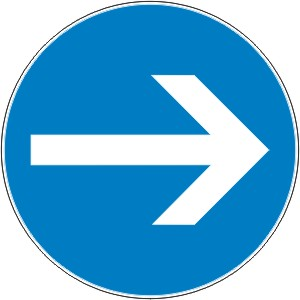
\includegraphics[scale=0.25]{figures/znak.png}
\caption{Predložak znaka obvezan smjer kretanja u desno upotrebljen za pronalazak.}
\label{fig:00}
\end{figure}

\begin{figure}[h]
\centering
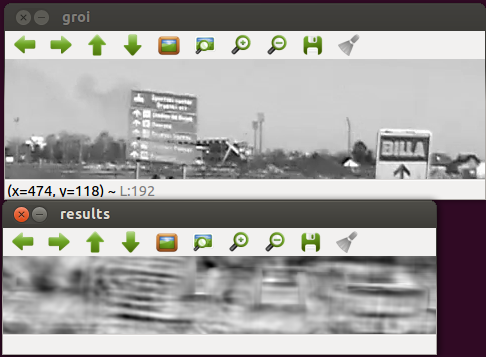
\includegraphics[scale=0.5]{figures/01.png}
\caption{Prikaz regije interesa i rezultata - pozitivan rezultat}
\label{fig:01}
\end{figure}

Lažno pozitivni rezultat prikazuje slika~\ref{fig:02} (lijevo) na kojoj 
je metoda
pronašala znak (iscrtala pravokutnik) gdje nije trebala. Takvi rezultati su očekivani ali nisu
poželjni te ih se pokušalo smanjiti na što manji broj metodom opisanom 
u podpoglavlju~\ref{ssub:Eliminacija lažno pozitivnih rezultata}

\begin{figure}[!htb]
\minipage{0.5\textwidth}
    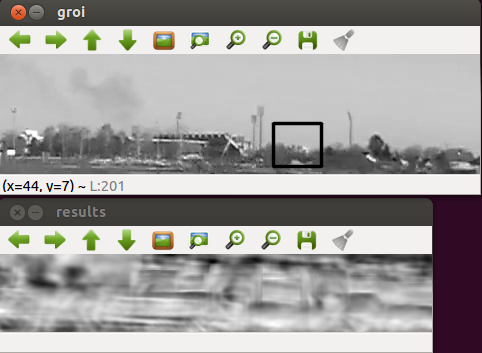
\includegraphics[width=\linewidth]{figures/02.png}
\endminipage\hfill
\minipage{0.5\textwidth}
    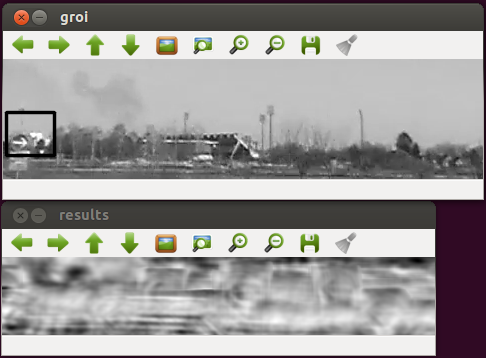
\includegraphics[width=\linewidth]{figures/03.png}
\endminipage\hfill
\caption{Prikaz regije interesa i matrice rezultata - negativan rezultat
(lijevo), pozitivan rezultat (desno).}
\label{fig:02}
\end{figure}


Na slici ~\ref{fig:04.png} (desno i lijevo) vidi se
da je metoda uspješno pronašla znak na različitim udaljenostima odnosno
veličinama znaka iako se koristila samo jedna veličina znaka za
pronalazak. Metoda odnosno program bi se mogao unaprijediti tako da se
ugradi uspoređivanje s različitim veličinama predloška odnosno znaka.

\begin{figure}[!htb]
\minipage{0.5\textwidth}
    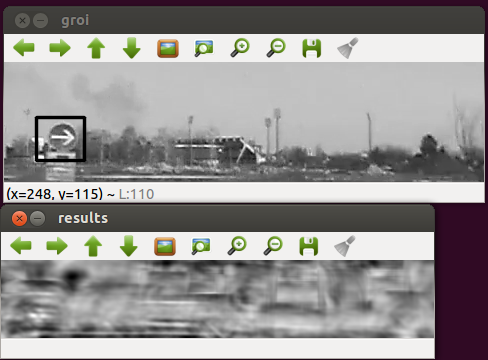
\includegraphics[width=\linewidth]{figures/04.png}
\endminipage\hfill
\minipage{0.5\textwidth}
    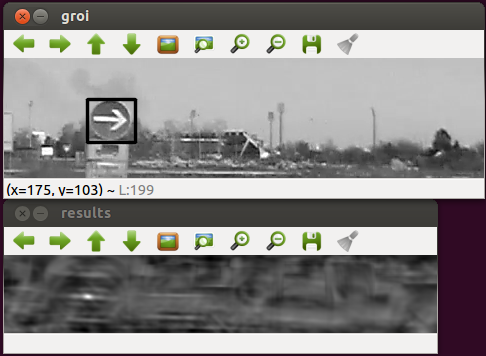
\includegraphics[width=\linewidth]{figures/05.png}
\endminipage\hfill
\caption{Prikaz regije interesa i matrice rezultata - pozitivan rezultat
(lijevo i desno).}
\label{fig:04.png}
\end{figure}

Matematička metoda korištena u algoritmu prikazuje pozitivne rezultate
bijelom bojom te se na slici~\ref{fig:04.png} jasno mogu vidjeti
"žarišta" u matrici rezultata.

\newpage

Slika~\ref{fig:06.png} (lijevo) također prikazuje uspješan pronalazak
znaka kada
je i znak na izvornoj slici nešto veći nego na slici predloška.
Slika~\ref{fig:06.png} (desno) prikazuje negativan rezultat iako se na slici s
rezultatima može vidjeti "žarište" na lokaciji gdje je znak. Program se
može unaprijediti da prati relativne vrijednosti u matrici rezultata i
na taj način bi se takvi negativni rezultati mogli smanjiti.

\begin{figure}[!htb]
\minipage{0.5\textwidth}
    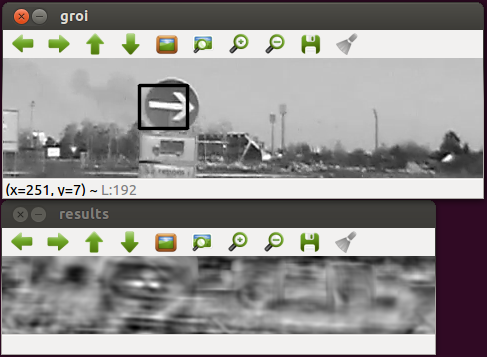
\includegraphics[width=\linewidth]{figures/06.png}
\endminipage\hfill
\minipage{0.5\textwidth}
    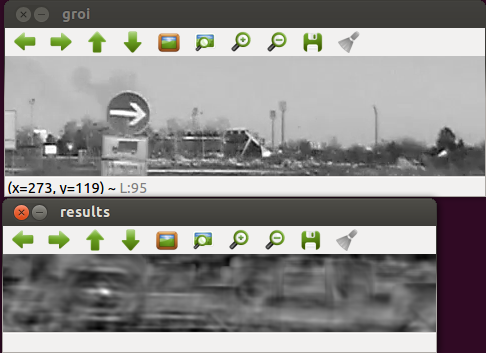
\includegraphics[width=\linewidth]{figures/07.png}
\endminipage\hfill
\caption{Prikaz regije interesa i matrice rezultata - pozitivan rezultat
(lijevo), negativan rezultat (desno).}
\label{fig:06.png}
\end{figure}

\newpage
\subsubsection*{Prikaz scene znak "obilaženje s obje strane"}

Osim scene sa znakom obvezan smjer kretanja u desno, program je pokrenut
nad još dvije scene. Prva je sa znakom obilaženje s obje strane. Na slikama 
\ref{fig:obz1}, \ref{fig:obz2} i \ref{fig:obz3} se vide regije interesa i 
izračunati rezultati odnosno pronađeni znak ukoliko postoji pravokutnik. Na
slici \ref{fig:obz4} se nalazi znak korišten kao predložak za pronalazak.

\begin{figure}[h]
\centering
\includegraphics[scale=0.4]{figures/znak2.jpg}
\caption{Predložak znaka obilaženje s obje strane upotrebljen za pronalazak.}
\label{fig:obz4}
\end{figure} 

\begin{figure}[!htb]
\minipage{0.5\textwidth}
    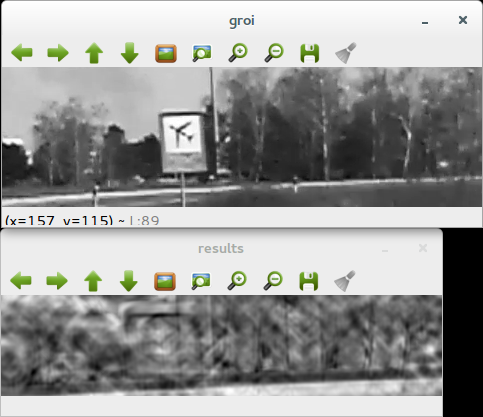
\includegraphics[width=\linewidth]{figures/08.png}
\endminipage\hfill
\minipage{0.5\textwidth}
    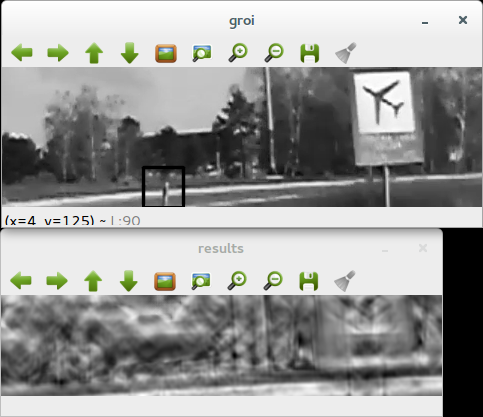
\includegraphics[width=\linewidth]{figures/09.png}
\endminipage\hfill
\caption{Prikaz regije interesa i matrice rezultata - pozitvan rezultat
(lijevo), negativan rezultat (desno).}
\label{fig:obz1}
\end{figure}


\begin{figure}[!htb]
\minipage{0.5\textwidth}
    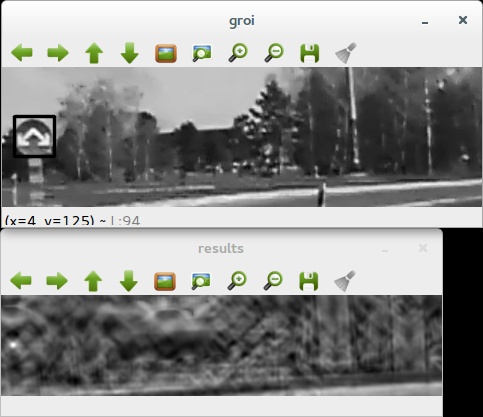
\includegraphics[width=\linewidth]{figures/10.png}
\endminipage\hfill
\minipage{0.5\textwidth}
    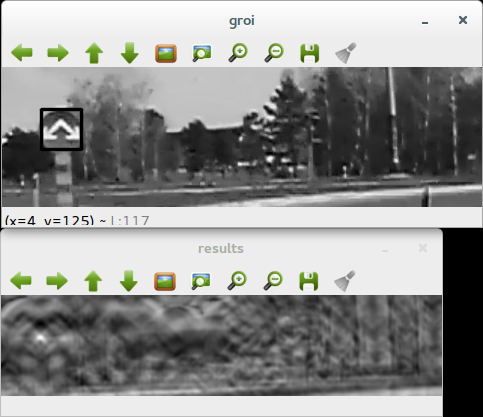
\includegraphics[width=\linewidth]{figures/11.png}
\endminipage\hfill
\caption{Prikaz regije interesa i matrice rezultata - pozitivan rezultat
 (lijevo i desno).}
\label{fig:obz2}
\end{figure}

\begin{figure}[!htb]
\minipage{0.5\textwidth}
    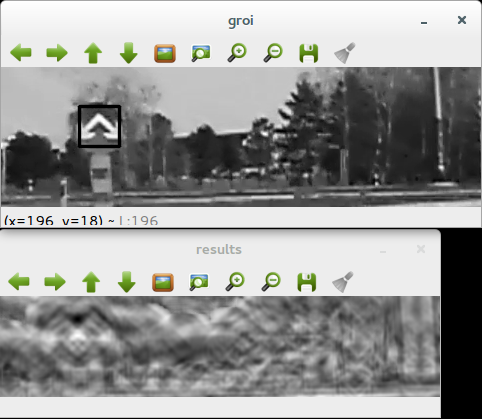
\includegraphics[width=\linewidth]{figures/12.png}
\endminipage\hfill
\minipage{0.5\textwidth}
    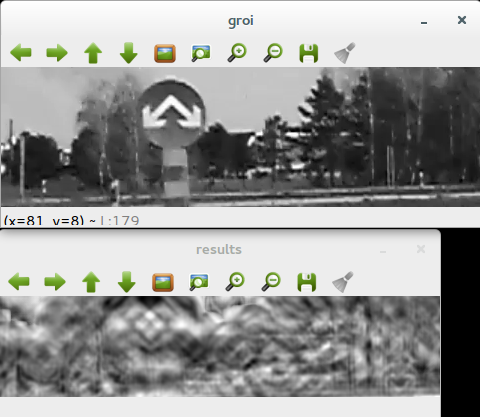
\includegraphics[width=\linewidth]{figures/13.png}
\endminipage\hfill
\caption{Prikaz regije interesa i matrice rezultata - pozitivan rezultat 
(lijevo), negativan rezultat (desno).}
\label{fig:obz3}
\end{figure}

\clearpage
\subsubsection*{Prikaz scene znak "prvenstvo prolaza"}

Na slikama \ref{fig:pr2}, \ref{fig:pr3} i \ref{fig:pr4} vide se 
regije interesa i izračunati rezultati odnosno pronađeni znak ukoliko postoji
pravokutnik. Slika \ref{fig:pr1} prikazuje predložak znak korišten za 
prepoznavanje.

\begin{figure}[!htb]
\centering
\includegraphics[scale=0.4]{figures/znak3.jpg}
\caption{Predložak znaka prvenstvo prolaza upotrebljen za pronalazak.}
\label{fig:pr1}
\end{figure} 

\begin{figure}[!htb]
\minipage{0.5\textwidth}
    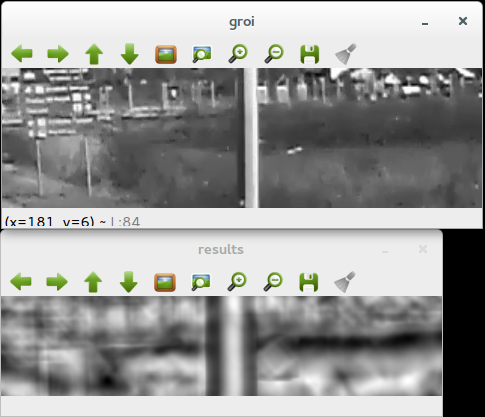
\includegraphics[width=\linewidth]{figures/14.png}
\endminipage\hfill
\minipage{0.5\textwidth}
    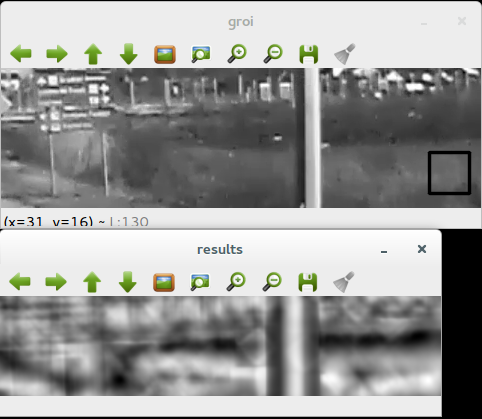
\includegraphics[width=\linewidth]{figures/15.png}
\endminipage\hfill
\caption{Prikaz regije interesa i matrice rezultata - pozitivan rezultat 
(lijevo), negativan rezultat (desno)}
\label{fig:pr2}
\end{figure}

\begin{figure}[!htb]
\minipage{0.5\textwidth}
    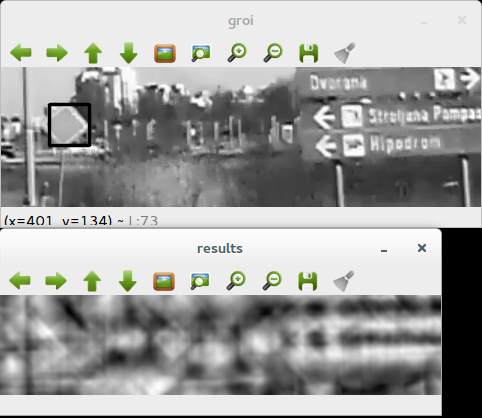
\includegraphics[width=\linewidth]{figures/16.png}
\endminipage\hfill
\minipage{0.5\textwidth}
    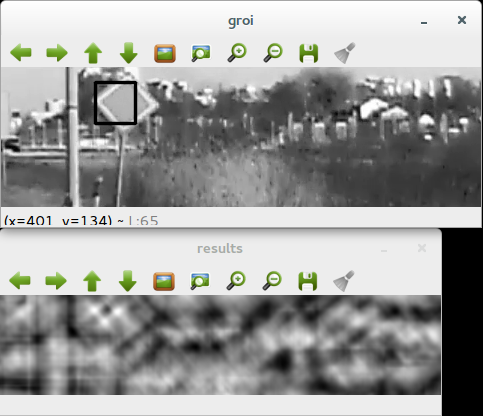
\includegraphics[width=\linewidth]{figures/17.png}
\endminipage\hfill
\caption{Prikaz regije interesa i matrice rezultata - pozitivan rezultat
(lijevo i desno)}
\label{fig:pr3}
\end{figure}

\begin{figure}[!htb]
\centering
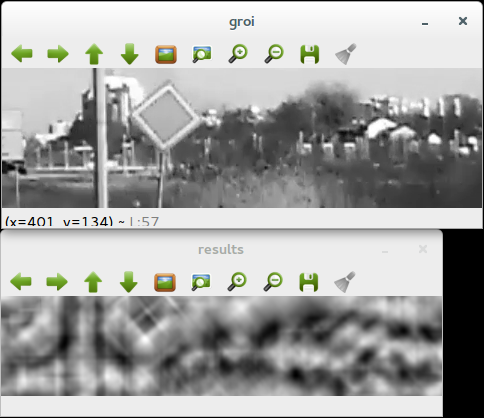
\includegraphics[scale=0.5]{figures/18.png}
\caption{Prikaz regije interesa i matrice rezultata - negativan rezultat}
\label{fig:pr4}
\end{figure}





% subsection Prikaz rezultata (end)
% section Rezultati (end)
